\section{Fuzzing third party apps} \label{sec:fuzzing}
\subsection{Introduction}
Static analysis of assembly code is a very time-consuming process that requires extensive knowledge.
Without any documentation, source code provided by the vendor, or any other help, it is extremely difficult to understand the code.

For this reason, I decided to use dynamic analysis to find vulnerabilities in the code.
As I am focusing on analysis of the virtual machine in the simulator, there are more possibilities to test the behaviour during runtime.
The simulator allows running the code in a controlled environment, which makes it easier to test different scenarios.
With this approach, there is no need to understand the code.
It is also valuable when the code base is large and complex.
Additionally, instead of spending time on reverse engineering, it is possible to write a fuzzer that will do the difficult work.
Sometimes it might be necessary to run the fuzzer for a long time.
This, however, does not require any human interaction and can be scaled to run on multiple machines or threads.
The expected outcome of the fuzzer is a binary file that crashes the virtual machine and can be run on the watch.

Finding vulnerabilities in the simulator is aimed at achieving two potential objectives.
Firstly, it might be possible to escape the sandbox and execute arbitrary code on the host machine.
Secondly, vulnerabilities in the simulator might be present in the real device as well.

\subsection{Environment setup}
When fuzzing a program, the most basic configuration would be to have a fuzzer and provide it with a program and the starting input.
Then the fuzzer would run the program with different modifications of the input and check if it crashes.

However, in this case, the setup is more complicated.
Simulator is run a standalone program.
Then the application has to be loaded with an additional command line script.
As such, the fuzzer needs to be aware of both tools.

Moreover, when modifying the input, the virtual machine requires it to be signed.
This means that to test the execution after each modification, the input needs to be signed again.


\subsection{Fuzzing solutions}
One of the most popular fuzzing solutions is AFL++\cite{aflplusplus}.
It is an improved fork to Google's AFL\footnote{\url{https://github.com/google/AFL}}, which is no longer maintained.
AFL++ is an open-source tool for fuzzing a wide range of software.
It is coupled with instrumentation-guided genetic algorithm, having a possibility to be extended for different use cases.

\subsection{Fuzzing process}
\begin{figure}[h]
    \centering
    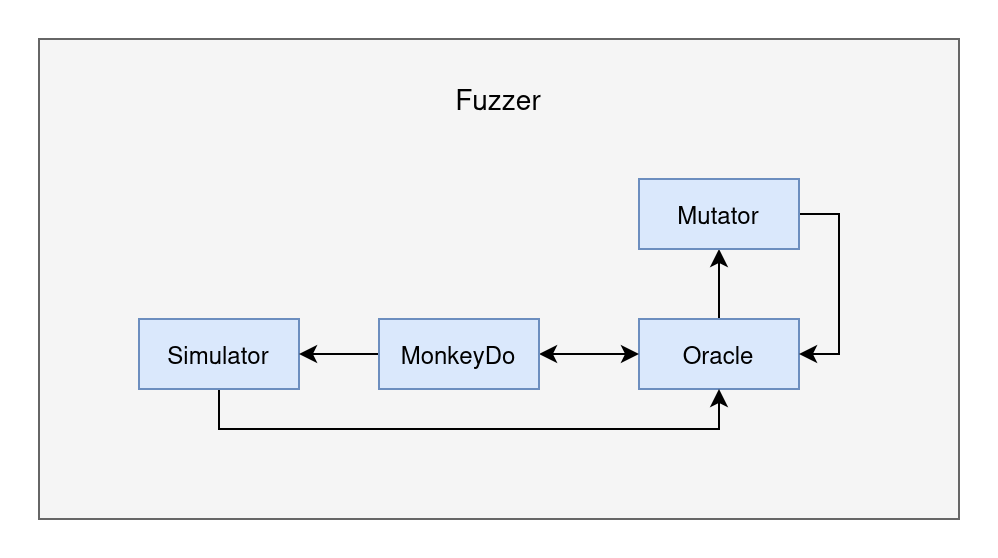
\includegraphics[width=0.8\linewidth]{../../images/fuzzer-diagram}
    \caption{Fuzzer diagram}
    \label{fig:fuzzer-diagram}
\end{figure}

The fuzzer consists of four main components: Mutator, Simulator, MonkeyDo, and Oracle.
The diagram of the fuzzer is presented in Figure~\ref{fig:fuzzer-diagram}.
\subsubsection*{Mutator}
\begin{lstlisting}[caption={Pseudocode of the mutating algorithm},captionpos=b,label={lst:mutator},language=Python]
originalApp = load("seed_app.prg")
currentApp = originalApp
lastMutation = emptyList()

def mutate(passed: Boolean):
    if passed:
        mutateCurrentApp()
    else:
        revertMutations()
    return sign(currentApp)

def mutateCurrentApp():
    mutation = generateMutation()
    for byte in mutation:
        currentApp[byte] = flipRandomBit(currentApp[byte])
    lastMutation = mutation

def revertMutations():
    lastMutation, bytesToRevert = splitInHalf(lastMutation)
    for byte in bytesToRevert:
        currentApp[byte] = originalApp[byte]

def generateMutation():
    mutationSize = mutationRate*len(currentApp)
    return [randomByte() for i in range(0, mutationSize)]
\end{lstlisting}

Mutator is responsible for generating a new input for the simulator.
It does that by mutating the original(seed) application.
The pseudocode of the mutating algorithm is presented in Listing~\ref{lst:mutator}.
Depending on the result of the previous execution, the mutator either mutates the current application or reverts the previous mutation.
To make the process more efficient, the mutator does not revert the whole mutation, but only half of it.
Using divide and conquer approach, it is possible to find the byte that broke the application faster.


\subsubsection*{Simulator}
\begin{figure}
    \centering
    \begin{subfigure}[b]{0.39\textwidth}
        \centering
        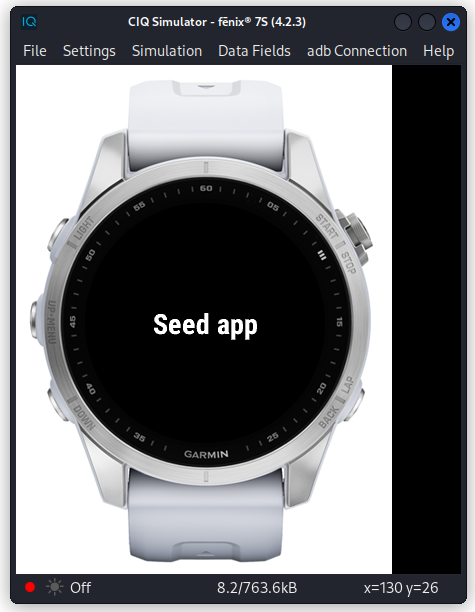
\includegraphics[width=1\linewidth]{../../images/simulator-seed-app}
        \caption{Simulator running seed app}
        \label{fig:simulator-seed-app}
    \end{subfigure}
    \begin{subfigure}[b]{0.6\textwidth}
        \centering
        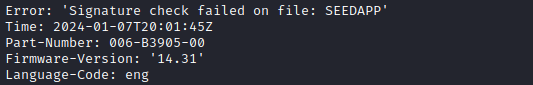
\includegraphics[width=1\linewidth]{../../images/simulator-signature-failed}
        \caption{Simulator output when signature verification fails}
        \label{fig:simulator-signature-failed}
    \end{subfigure}
\end{figure}
The simulator component is responsible for running the simulator executable.
It monitors the output of the simulator to recognise if the provided input has been executed successfully.
This information is needed to decide if the mutator should mutate the current application or revert the previous mutation.
Additionally, it detects when the simulator crashes.
This information is used by the Oracle component to decide if a bug has been found.

\subsubsection*{MonkeyDo}


\subsubsection*{Oracle}

\subsection{Fuzzing results}

\begin{figure}[h]
    \centering
    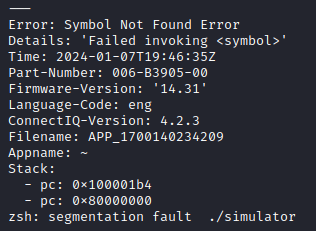
\includegraphics[width=0.4\linewidth]{../../images/simulator-crash}
    \caption{Simulator crash}
    \label{fig:simulator-crash}
\end{figure}